\begin{figure}[htbp]
\centering
\begin{tikzpicture}[x=1cm,y=1cm]
\node[anchor=south west,inner sep=0] at (0,0) {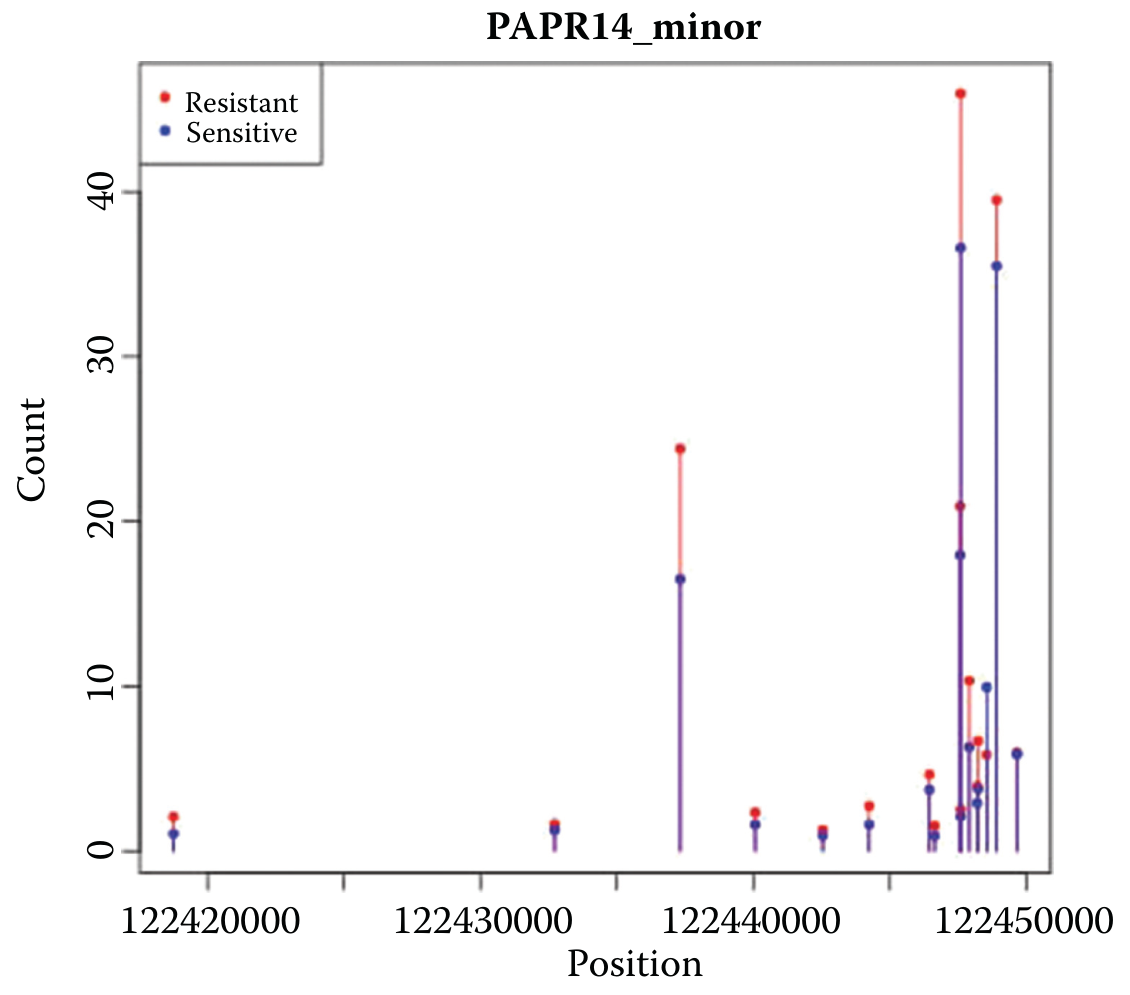
\includegraphics[width=9.8cm]{figures/ch04a_fig17_data.png}};
\fill[white] (4.8892,0.0574) rectangle (6.1237,0.4543);
\node[inner sep=0pt,fill=white,rotate=0,font=\fontsize{8}{8}\selectfont] at (5.5064,0.2558) {位置};
\fill[white] (0.0980,4.2398) rectangle (0.4949,5.2039);
\node[inner sep=0pt,fill=white,rotate=90,font=\fontsize{8}{8}\selectfont] at (0.2964,4.7219) {计数};
\fill[white] (1.5746,7.5693) rectangle (2.6135,7.8794);
\node[inner sep=0pt,fill=white,rotate=0,font=\fontsize{8}{8}\selectfont] at (2.0940,7.7243) {耐药};
\fill[white] (1.5895,7.3089) rectangle (2.6050,7.6191);
\node[inner sep=0pt,fill=white,rotate=0,font=\fontsize{8}{8}\selectfont] at (2.0972,7.4640) {敏感};
\fill[white] (4.1853,8.1811) rectangle (6.6292,8.5780);
\node[inner sep=0pt,fill=white,rotate=0,font=\fontsize{8}{8}\selectfont] at (5.4073,8.3795) {PAPR14：次要等位基因};
\end{tikzpicture}
\origfig{17}{基因 PAPR14 次要等位基因的差异表达。}
\label{fig:ch04a-17}
\end{figure}
